\section{Wire Connectivity Tests}
\label{sec:TheTest}

The main goal of the ICARUS TPC's connectivity tests here described has been to check the condition of the wires of the each anode plane of the detector; i.e., to look/check for wires not properly working or even disconnected. \\

The tests, as described in \cref{ssec:stand_chimn}, were done using a test box that sends a pulse of specific voltage, triggers the oscilloscope and receives back an output signal from the wires and sends it to oscilloscope where we can look and measure the expected peak and amplitude.\\

Since horizontal cables can't get a pulse injected, there was a slightly different procedure to test the 8 non-standard chimneys (See \cref{ssec:nonStd_chimn}). 


\subsection{Test box}
\label{ssec:TestBox}

The SLAC test box (Fig.) was designated specially for the ICARUS TPC wire plane connectivity tests. It's a portable battery powered device with dimensions $20\times 15\times 10$ cm.\\

\begin{figure}[htb]
\centering
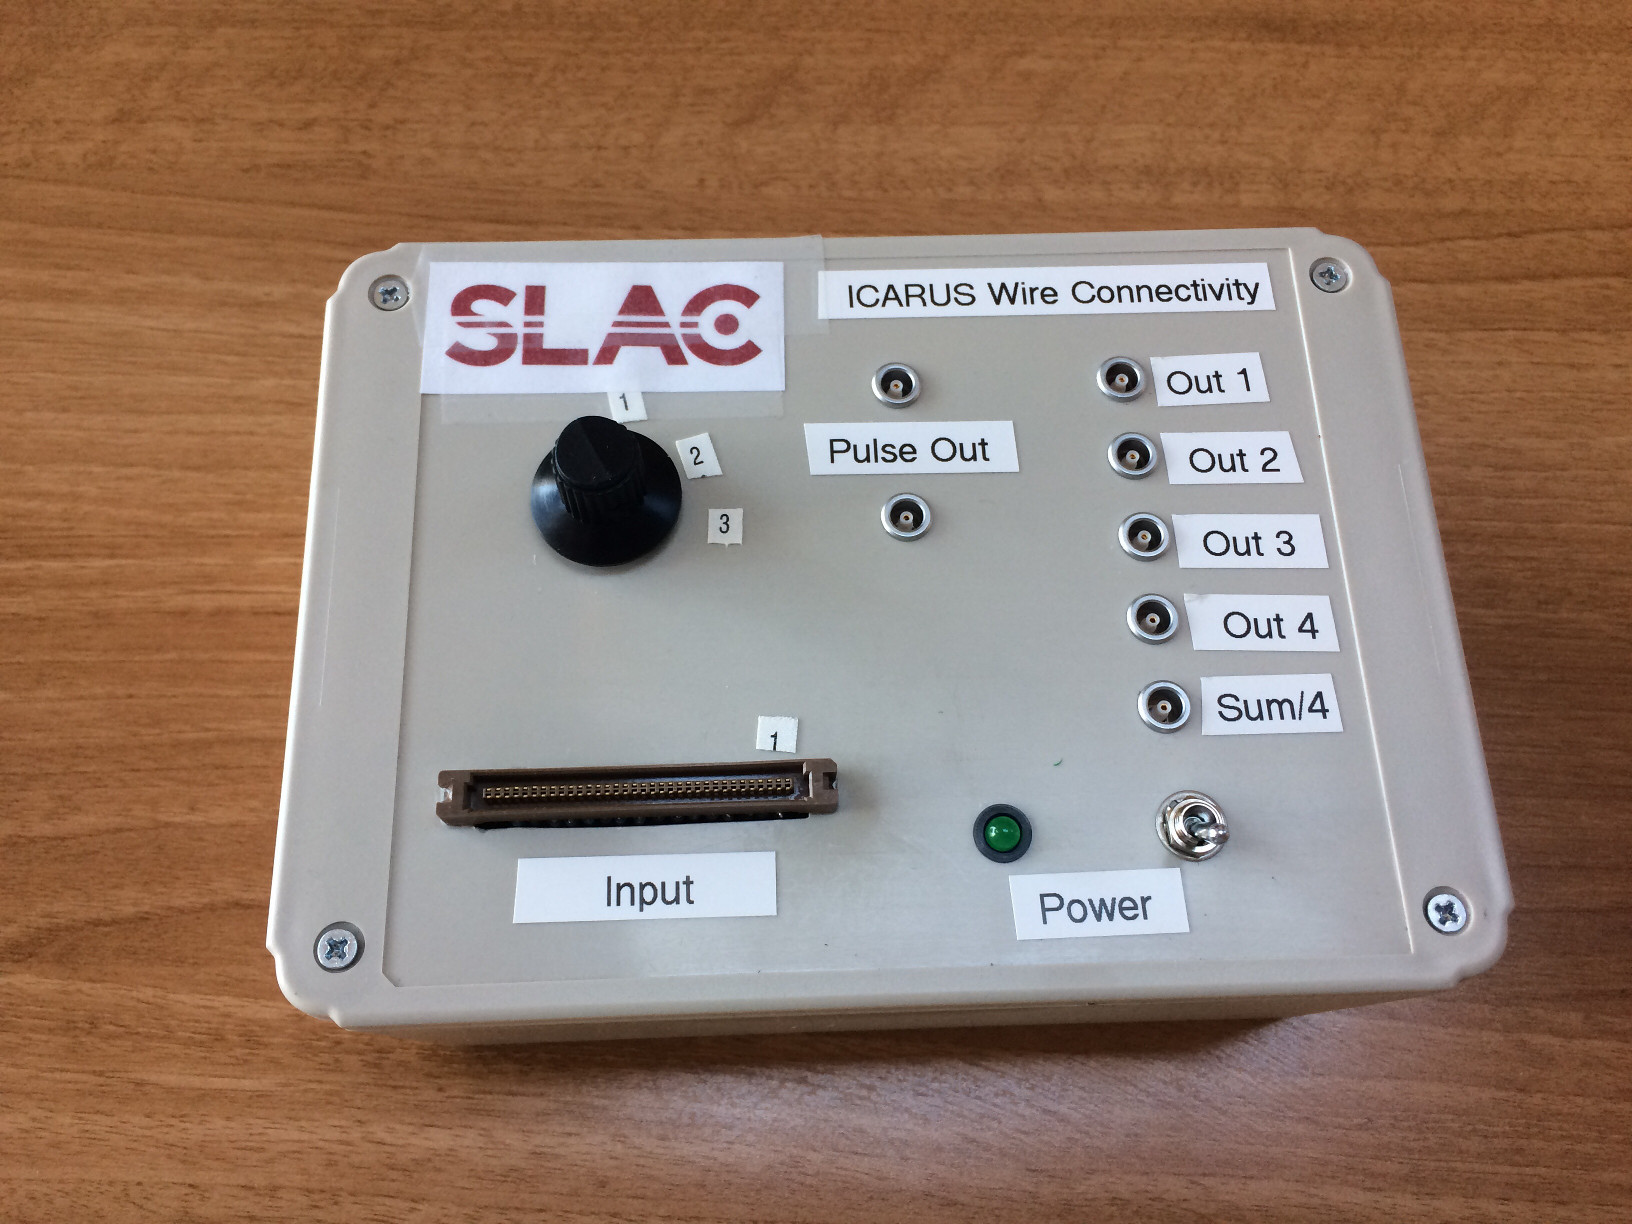
\includegraphics[width=0.8\linewidth]{fig/box1}
\caption{SLAC test box version 1}
\end{figure}

On the lid it contains:
\begin{itemize}
\item Built in pulser outputs on LEMO with both polarities,
\item Connector for a single flat ribbon of twisted-pairs cable: TPC cables plug into this connector with all grounds connected together.
\item An 8-position rotary switch that switches all 4 channels at a time,
\item The test pulse: $100$ Hz, $5$ V, $1 \mu $s rise time, $100 \mu $s length.

Two test boxes were built. It was found out that the cable shields, although connected together, were not grounded in the box. This was observed as a full size signal of about $1.5$ V.  The second version of the box contains extra outputs that allowed us to ground the shields of the connectors (Fig. second box). 
\end{itemize}

%SPEND MORE WORDS (regarding schematics of the electronics inside) ON THE TEST BOX!!!!



\subsection{Standard Chimneys}
\label{ssec:stand_chimn}

%The standard chimneys of the detector are the 2 to 19 $1$m tall cylinders that are bolted to the flanges on top of the cryostats (Fig.).

%\begin{figure}[H]
%\centering
%\includegraphics[scale=0.1]{fig/chimn}
%\caption{Chimneys installed, view from south to north.}
%\end{figure}

The TPC cables were pulled out from the detector through all the chimneys (Fig.) and the tests were performed in the following way: \\


%THIS PARAGRAH/INFO goes in Part II.
%The standard chimneys contain $18$ flat ribbon connectors each, $8$ pulser cables, groups of cables that belongs to the photomultipliers (High Voltage and signal) and optical fibers.\\

%\begin{figure}[H]
%\centering
%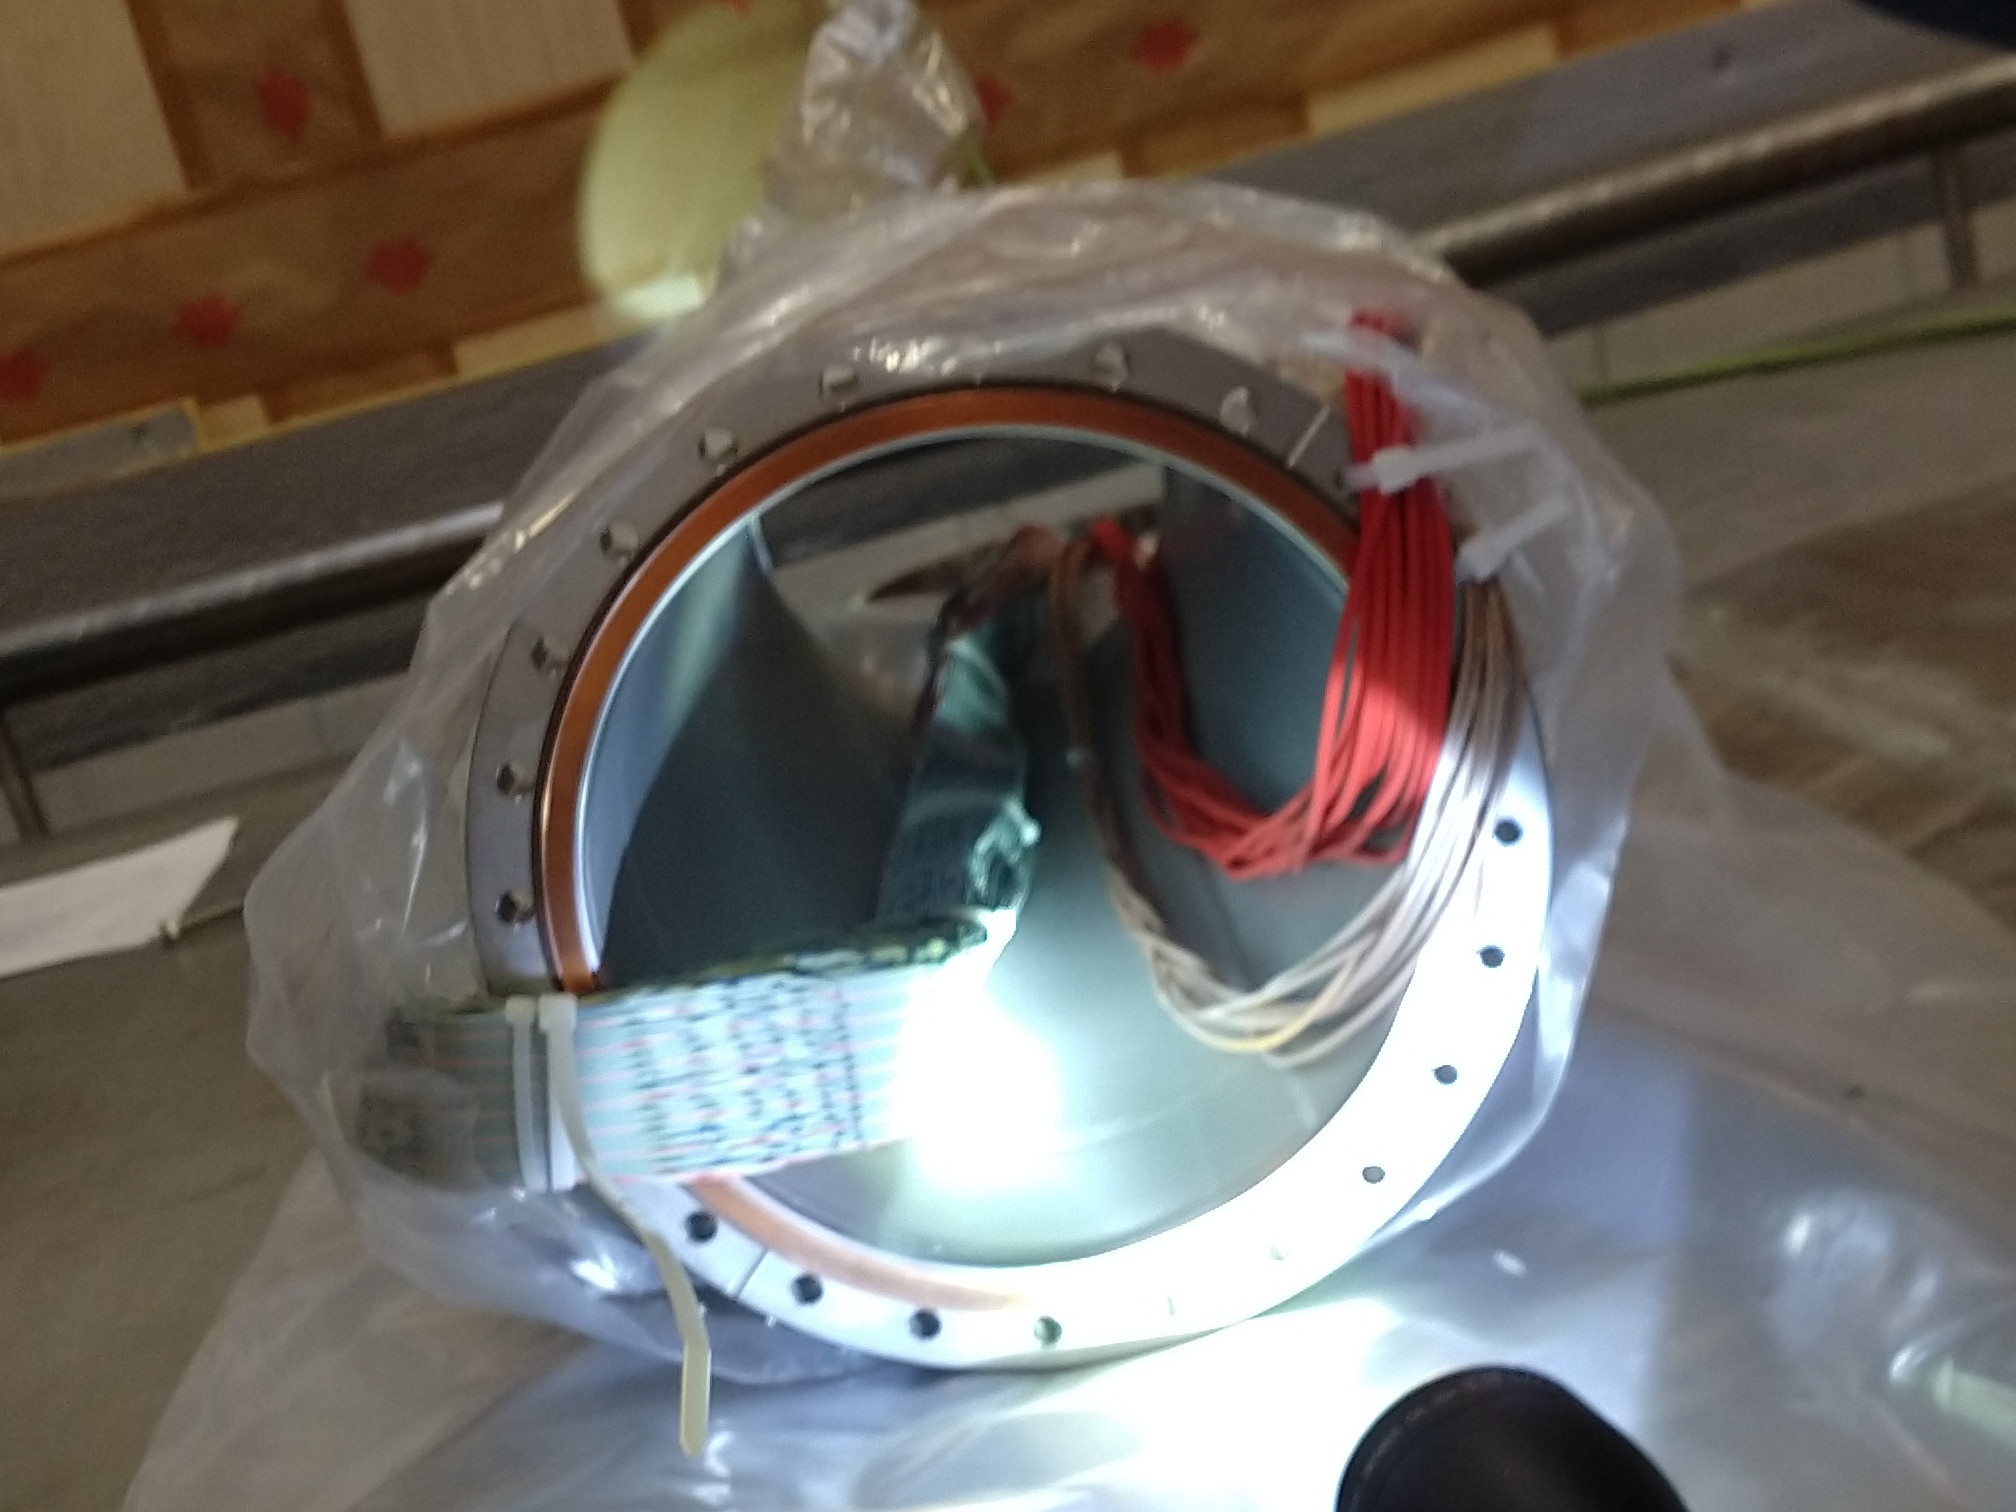
\includegraphics[scale=0.06]{fig/cab1} 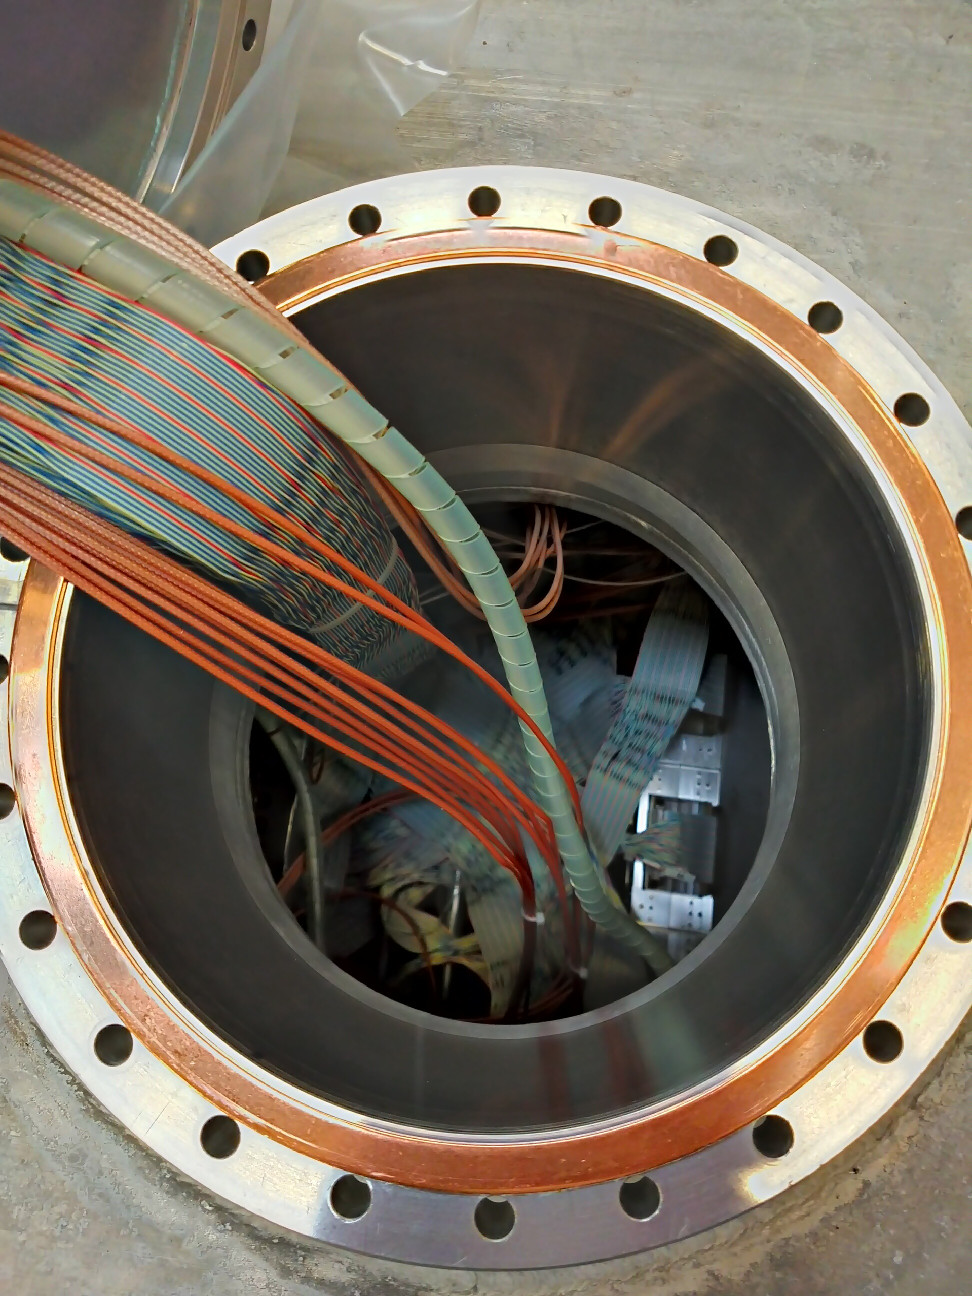
\includegraphics[scale=0.08]{fig/cab2}
%\caption{Left: Installation of a chimney. Right: HV PMT's cables (red), TPC connectors (colored flat ribbon cables)}
%\end{figure}


%Also this lines go in Part II
%The cables of interest are:
 
%\begin{itemize}
%\item 4 of the 8 SMA cables, the ones with red tag,

%\begin{figure}[H]
%\centering
%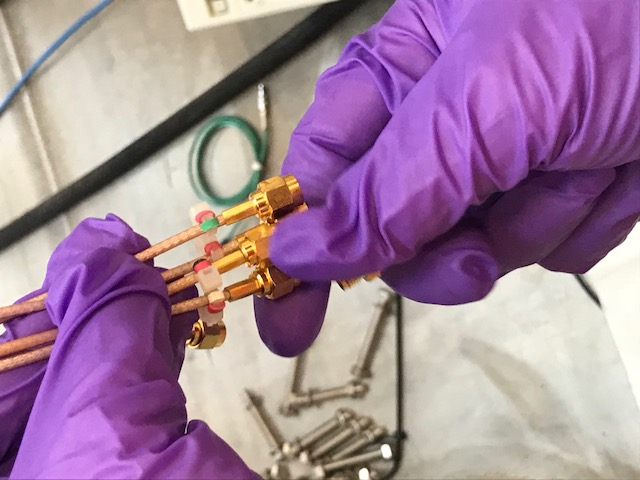
\includegraphics[scale=0.3]{fig/SMA} 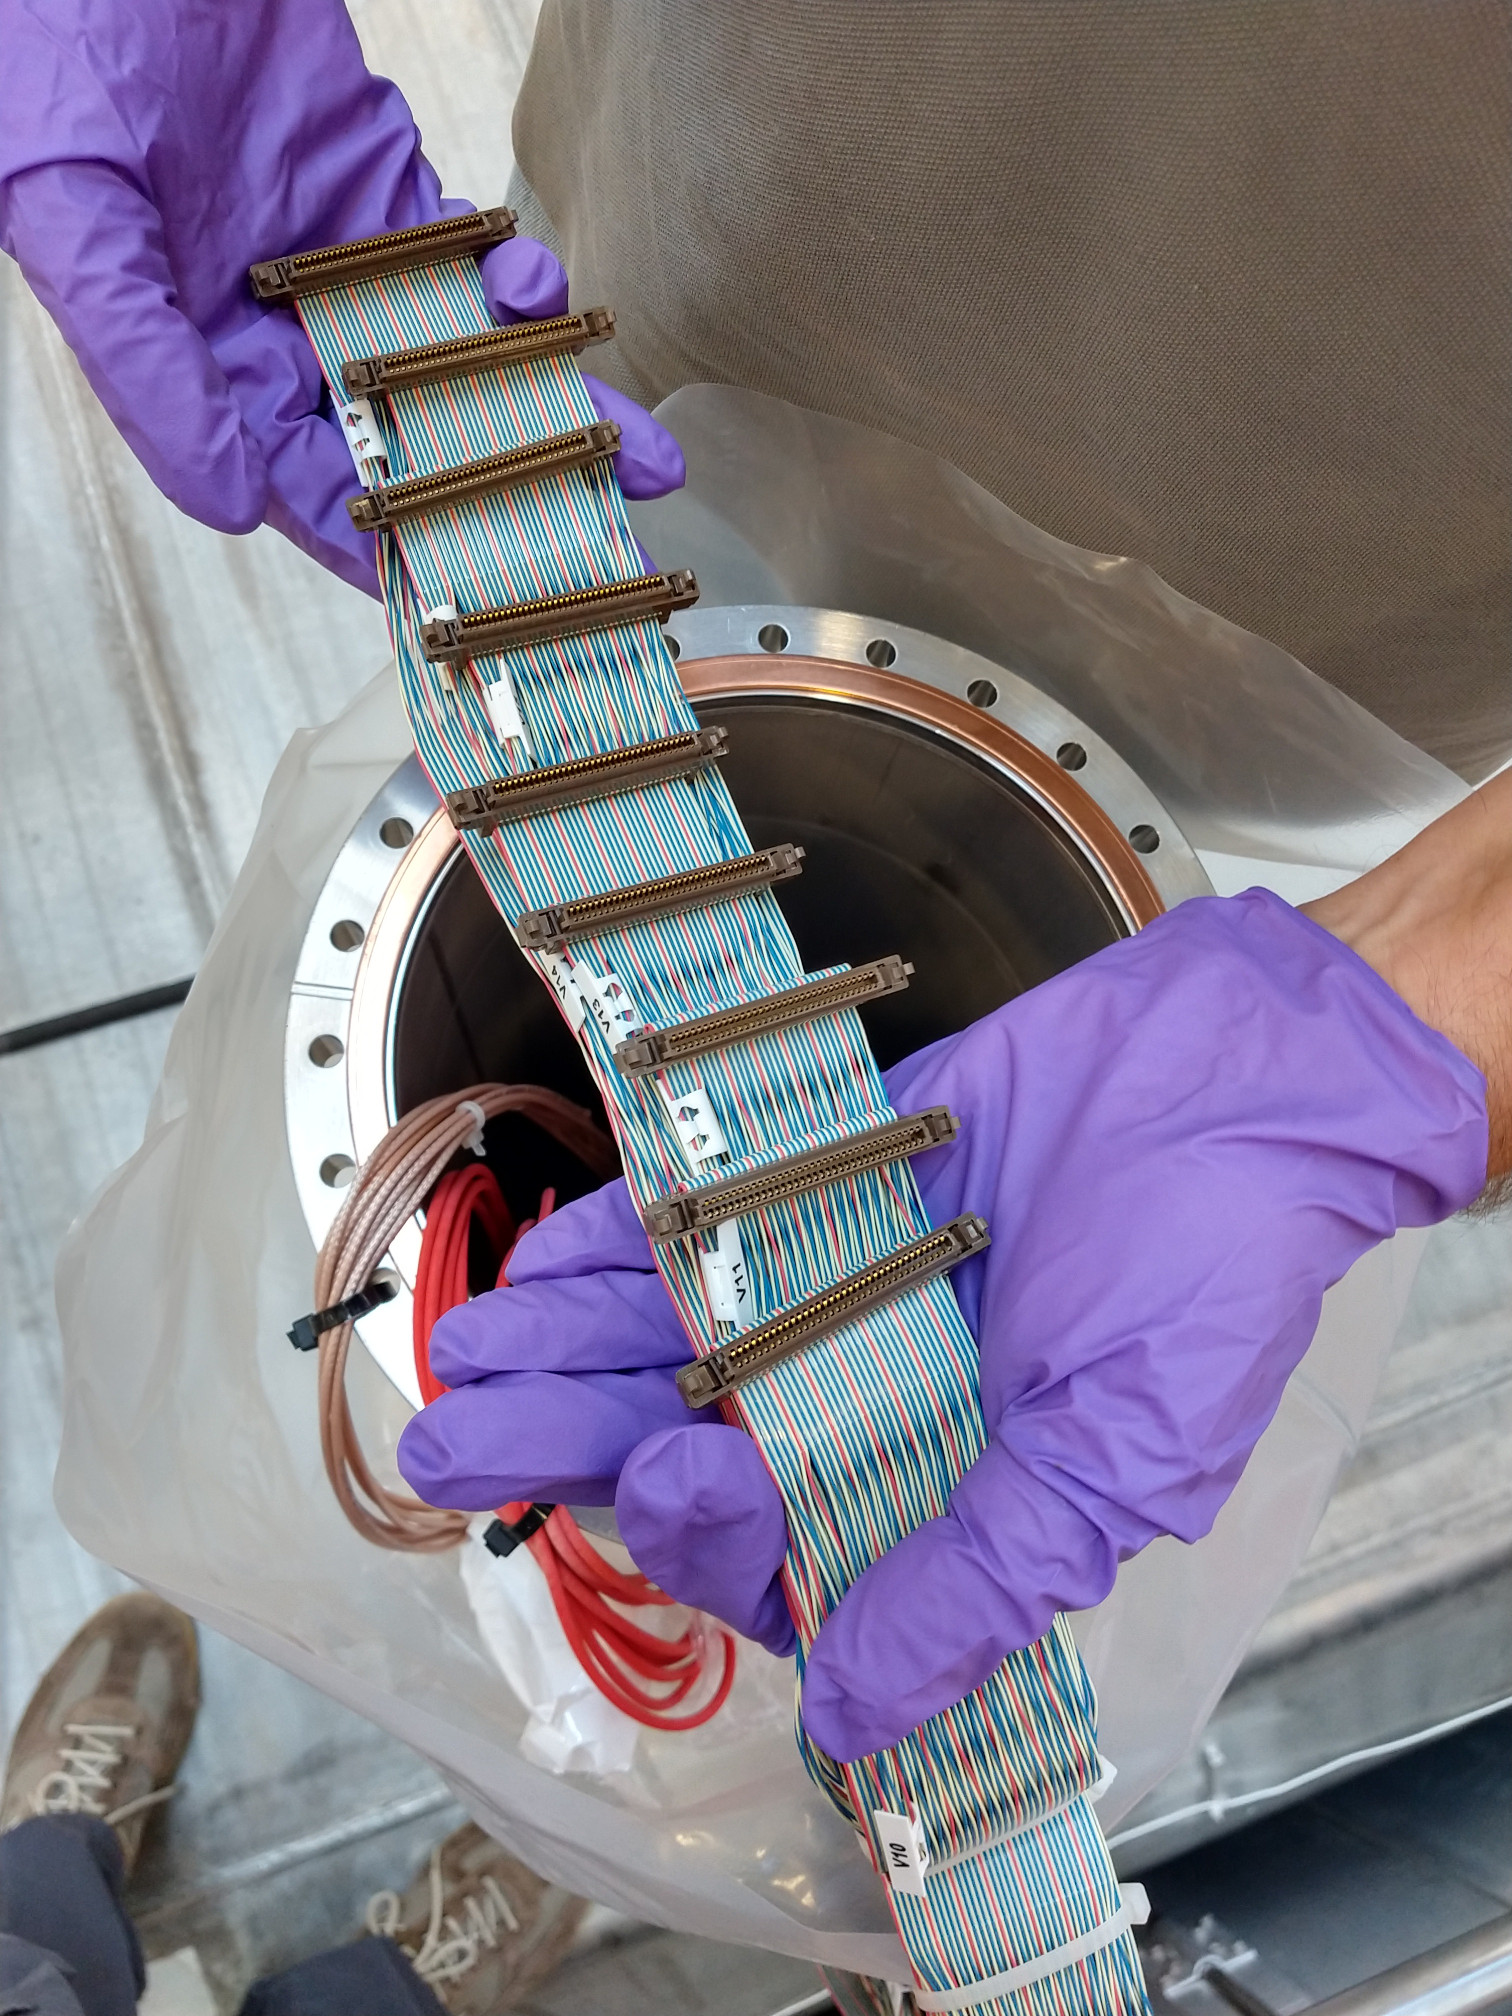
\includegraphics[scale=0.05]{fig/conn1}
%\caption{Left: SMA pulser cables, Right: 32 TPC wires per each single flat ribbon of twisted-pairs cables.}
%\end{figure}

%\item the $18$ flat ribbon connectors.

%\end{itemize}

\textit{Procedure:}\\
\begin{enumerate}
\item The external trigger was connected from one of the test-pulse output of the box to the oscilloscope (at the back). Therefore, the setting for the trigger in the oscilloscope input was changed to: "EXT" (external).

\item 4 LEMO cables connected from the box to the four inputs of the oscillope correspond to four channels of the signal (Fig.).

\item A SMA-female coaxial cable goes connected on the "pulse-out" of the box via LEMO conection and the SMA-female side is connected to the pulser from the detector.

An important requirement before starting to take data was to test all 4 SMA cables (red tag) in the search for the highest pulse.

In order to verify that everything was working properly, the box was tested in-site by connecting the test-pulse output directly to one channel of the oscilloscope, with the settings changed to DC and $1$ M$\Omega $ and looked for the $5$ V square signal on the screen. In addition, we verified the SMA (from the detector) to LEMO (pulser cable from the box) connection by using a chain of LEMO to SMA-female plus SMA-male to LEMO to connect the test box to the oscilloscope.

\item For a systematic test, we chose to start from the cable S/V18 to S/V1. Since the test box injects and receives output signal from only 4 cables of a single flat ribbon connector, we had to swith through 8 positions with the black know on top of the box in order to test all 32 wires from 1 connector at a time. 

\item The waveforms seen on the screen of the oscilloscope were downloaded using a Python script written by S. Castells [ref] and stored in an external disk for an offsite analysis. 


\begin{figure}[H]
\centering
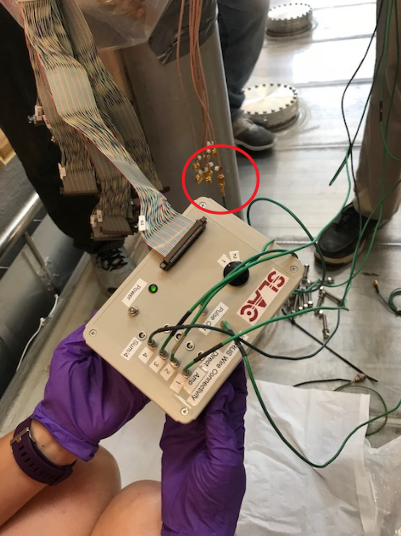
\includegraphics[scale=0.6]{fig/setup}
\caption{Set up of the hardware components. The red circle shows the SMA to LEMO connectors through which the box injects the test pulse.}
\end{figure}




\end{enumerate}




\subsection{Non-standard chimneys}
\label{ssec:nonStd_chimn}

The non-standard chimneys are the 8 corners of both cryostats, see Fig. Apart from the difference in size between standard and non-standard chimneys, the latter ones contain the horizontal and corner wire connectors. \\

As described on \cref{sec:Detector} the configuration of the horizontal wires does not allow to inject a pulse directly to the wires and therefore a different way to test them was developed. \\
The test pulse was injected to 32 wires of Induction-2 plane at once. From one standard chimney, two or three chimneys away from the corner, a connector between 2 and 9 was choosen and plugged in to a board (<-name?). To pulse those 32 wires we use the same conexion from the test box: a chain LEMO to SMA cables and to one of the 4 red-tagged pulser cables from the chimney.  


\subsection{Waveforms retrieval}
\label{ssec:DAQ}

I will add the procedure for the retrieval and the code used?

